\documentclass[10pt,aspectratio=149]{beamer}
\usecolortheme{Calm}
\usetheme{Calm}
\usepackage{pgfplots}
\usepackage{pgfplotstable}
\usepackage[utf8]{inputenc}
\usepackage{hyperref}
\RequirePackage[absolute,overlay]{textpos}
%\usepackage[sfdefault]{cabin}
%\usepackage[T1]{fontenc}
%\setlength{\TPHo{}rizModule}{\paperwidth}
%\setlength{\TPVertModule}{\paperheight}
%\definecolor{OQEdarkblue}{HTML}{046085}


\defbeamertemplate*{background canvas}{bg}
{%
  \color{lightgray!40}\vrule width\paperwidth height\paperheight% added bg color
}

%------------------------------

\author{Dominique Gravel}
\title{Introduction}
\date{August 24th, 2026}
\institute{Université de Sherbrooke \\ Summer school in biodiversity modelling}

%------------------------------
% TITLE SLIDE
%------------------------------

\usebackgroundtemplate
{
  
\includegraphics[width=\paperwidth,height=\paperheight]{bg}%
}

\begin{document}

	\begin{frame}[plain]
		\titlepage
	\end{frame}

%------------------------------
% INTRODUCTION
%------------------------------

\begin{frame}{Individual movement}

    \begin{center}
        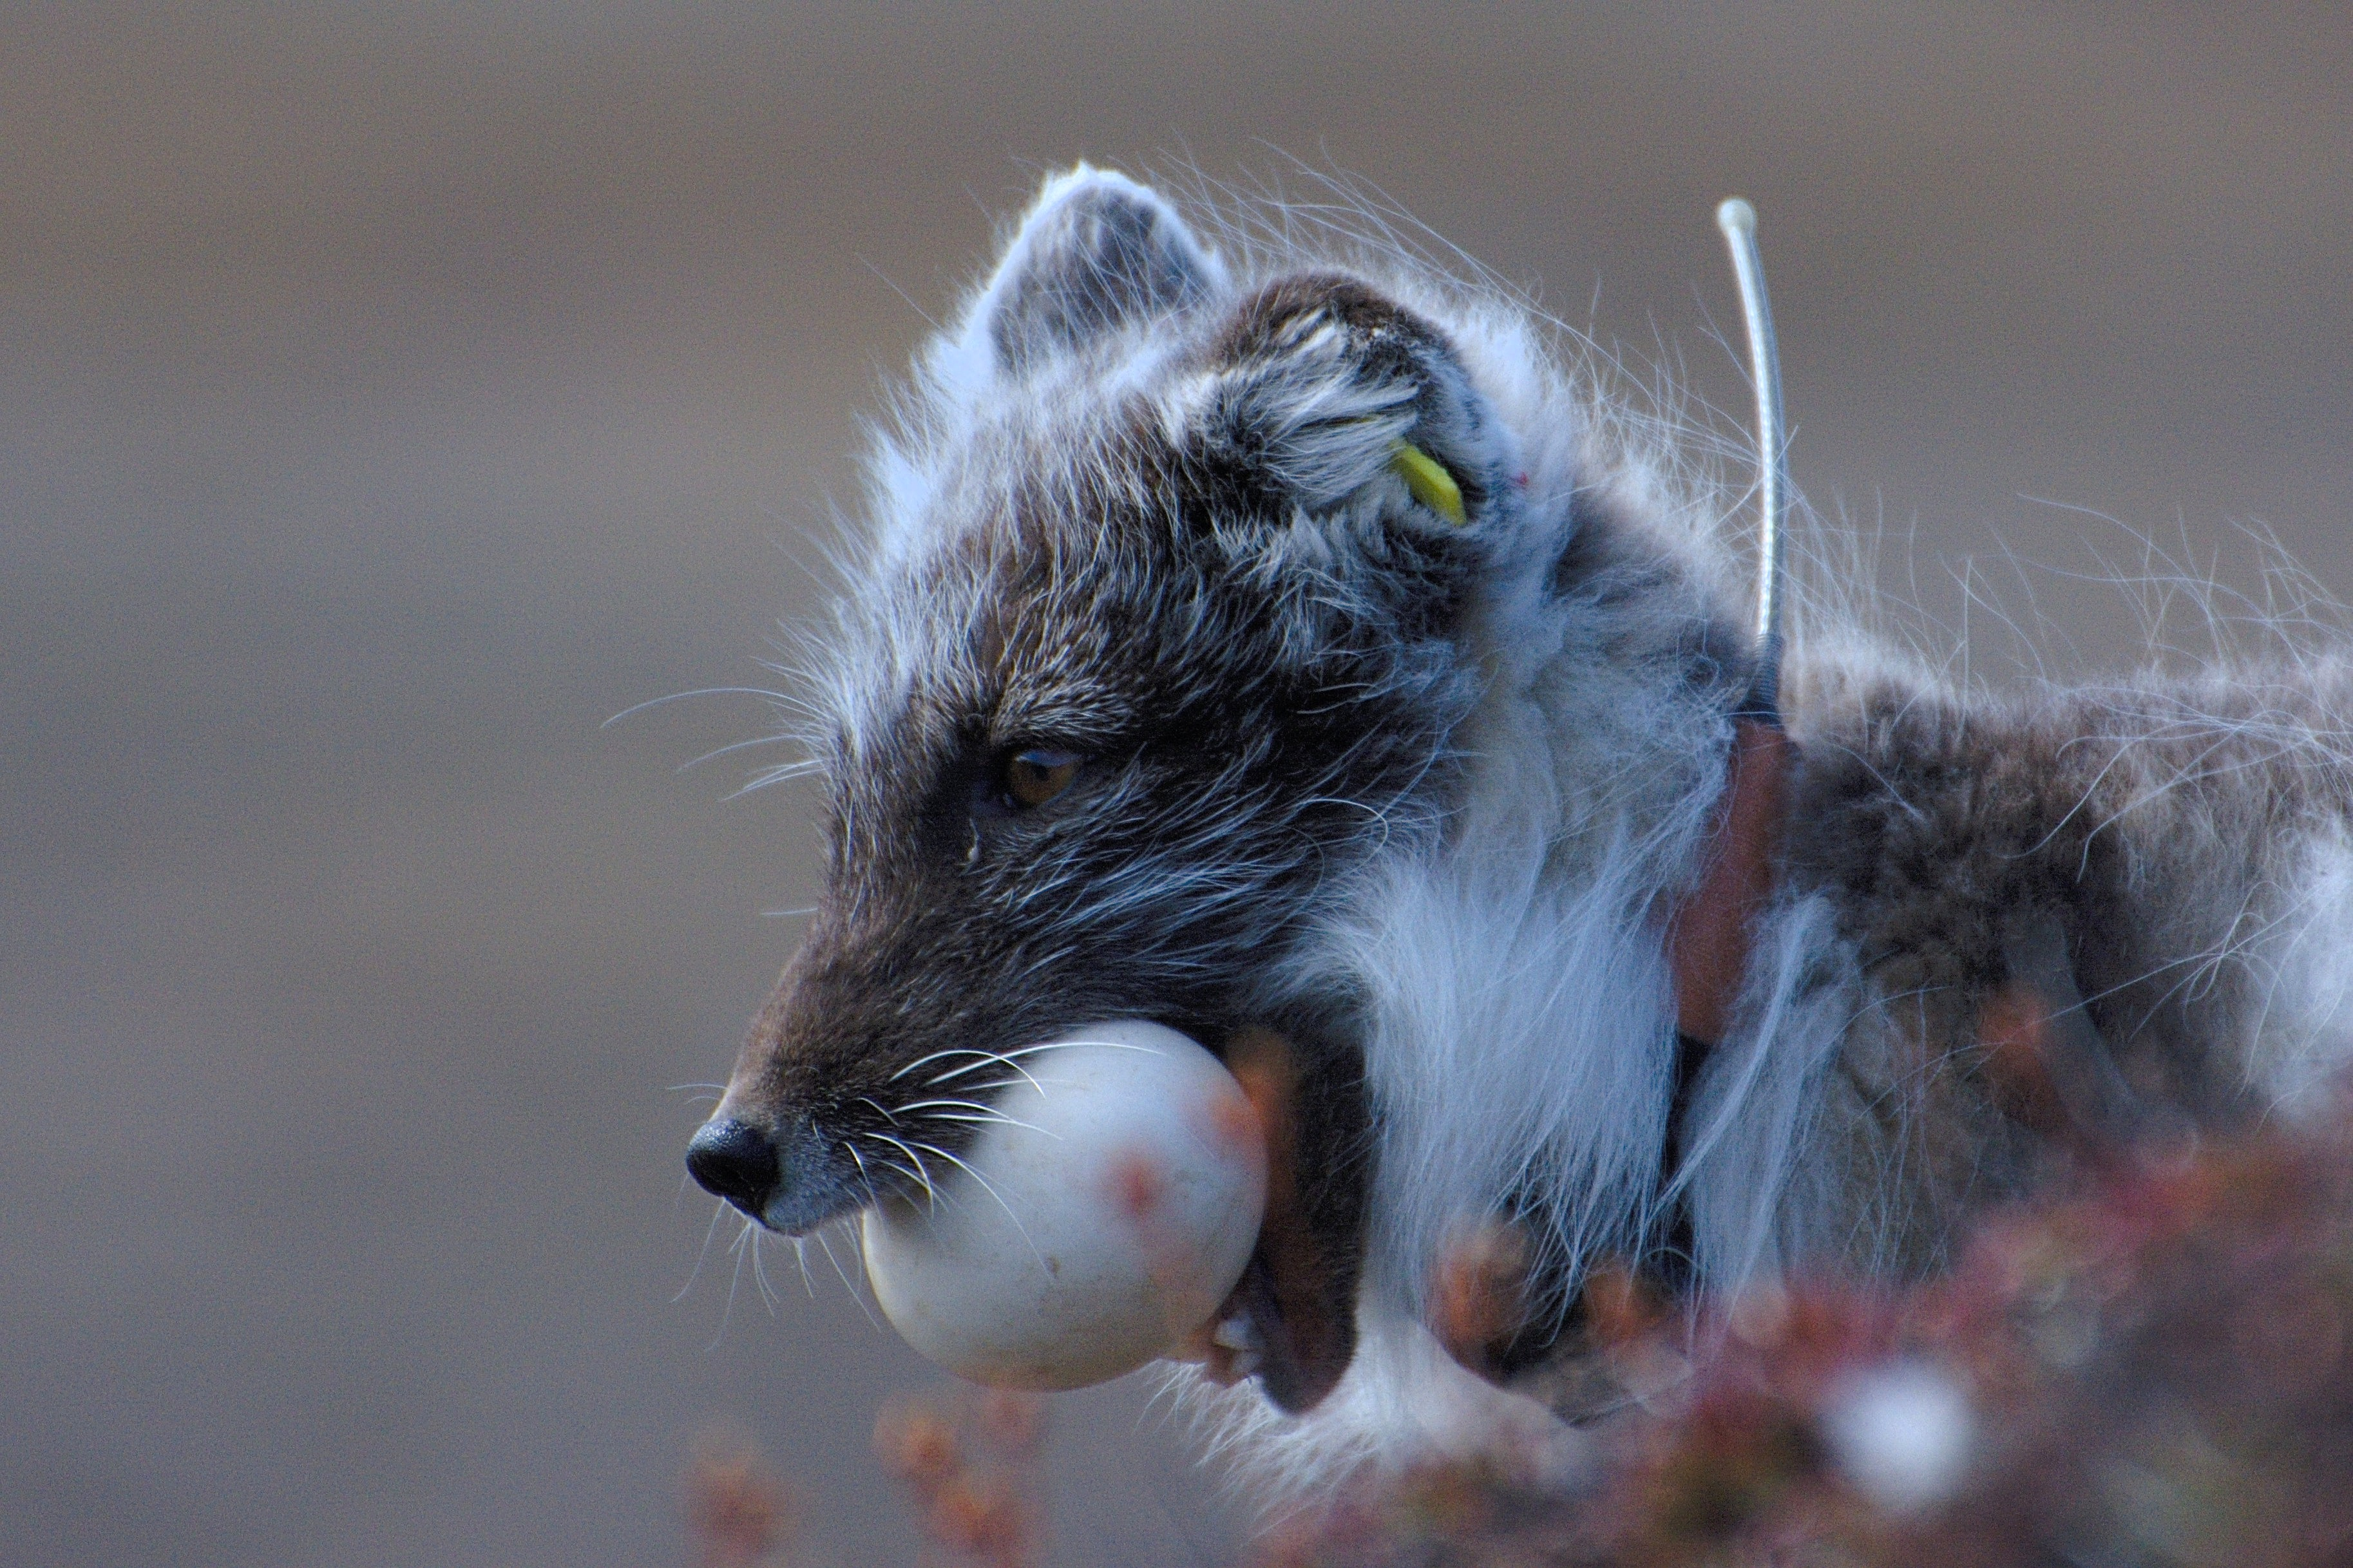
\includegraphics[height=0.7\textheight]{Figs/fox}
    \end{center}

\end{frame}

%------------------------------

\begin{frame}{Home range}

    \begin{center}
        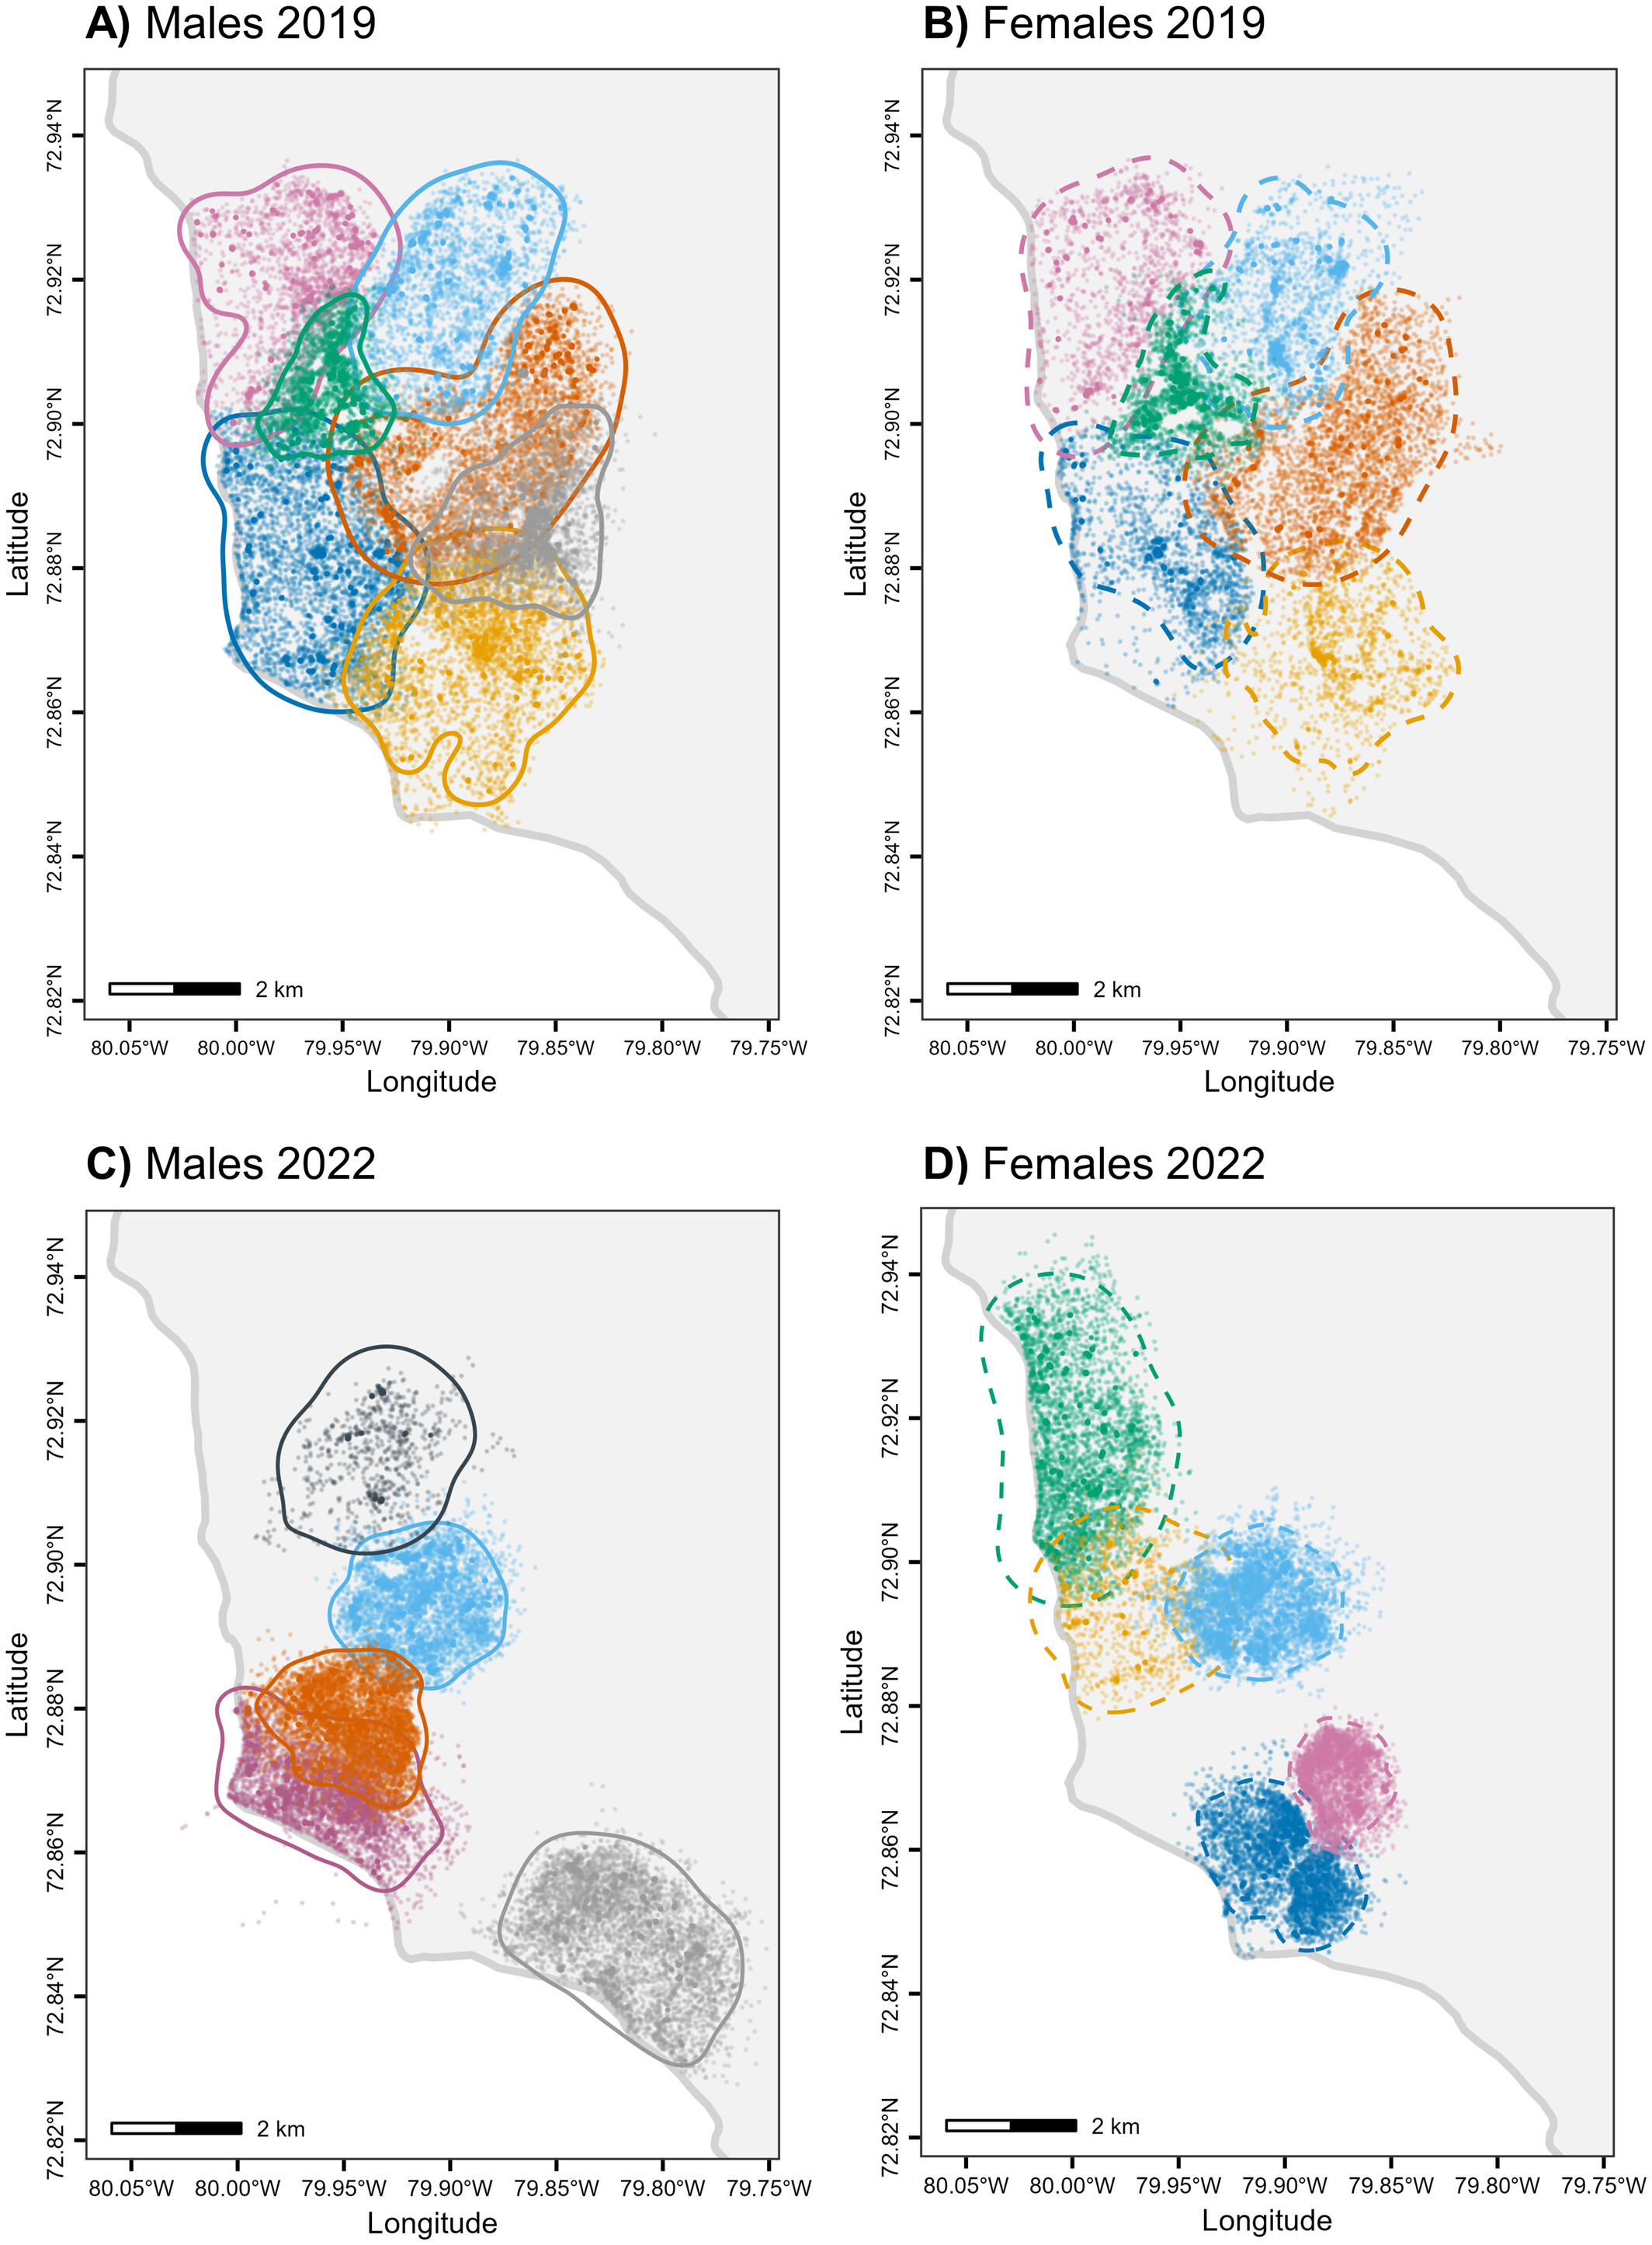
\includegraphics[height=0.8\textheight]{Figs/home_range_fox}
    \end{center}

\end{frame}

%------------------------------

\begin{frame}{Gradients}

    \begin{center}
        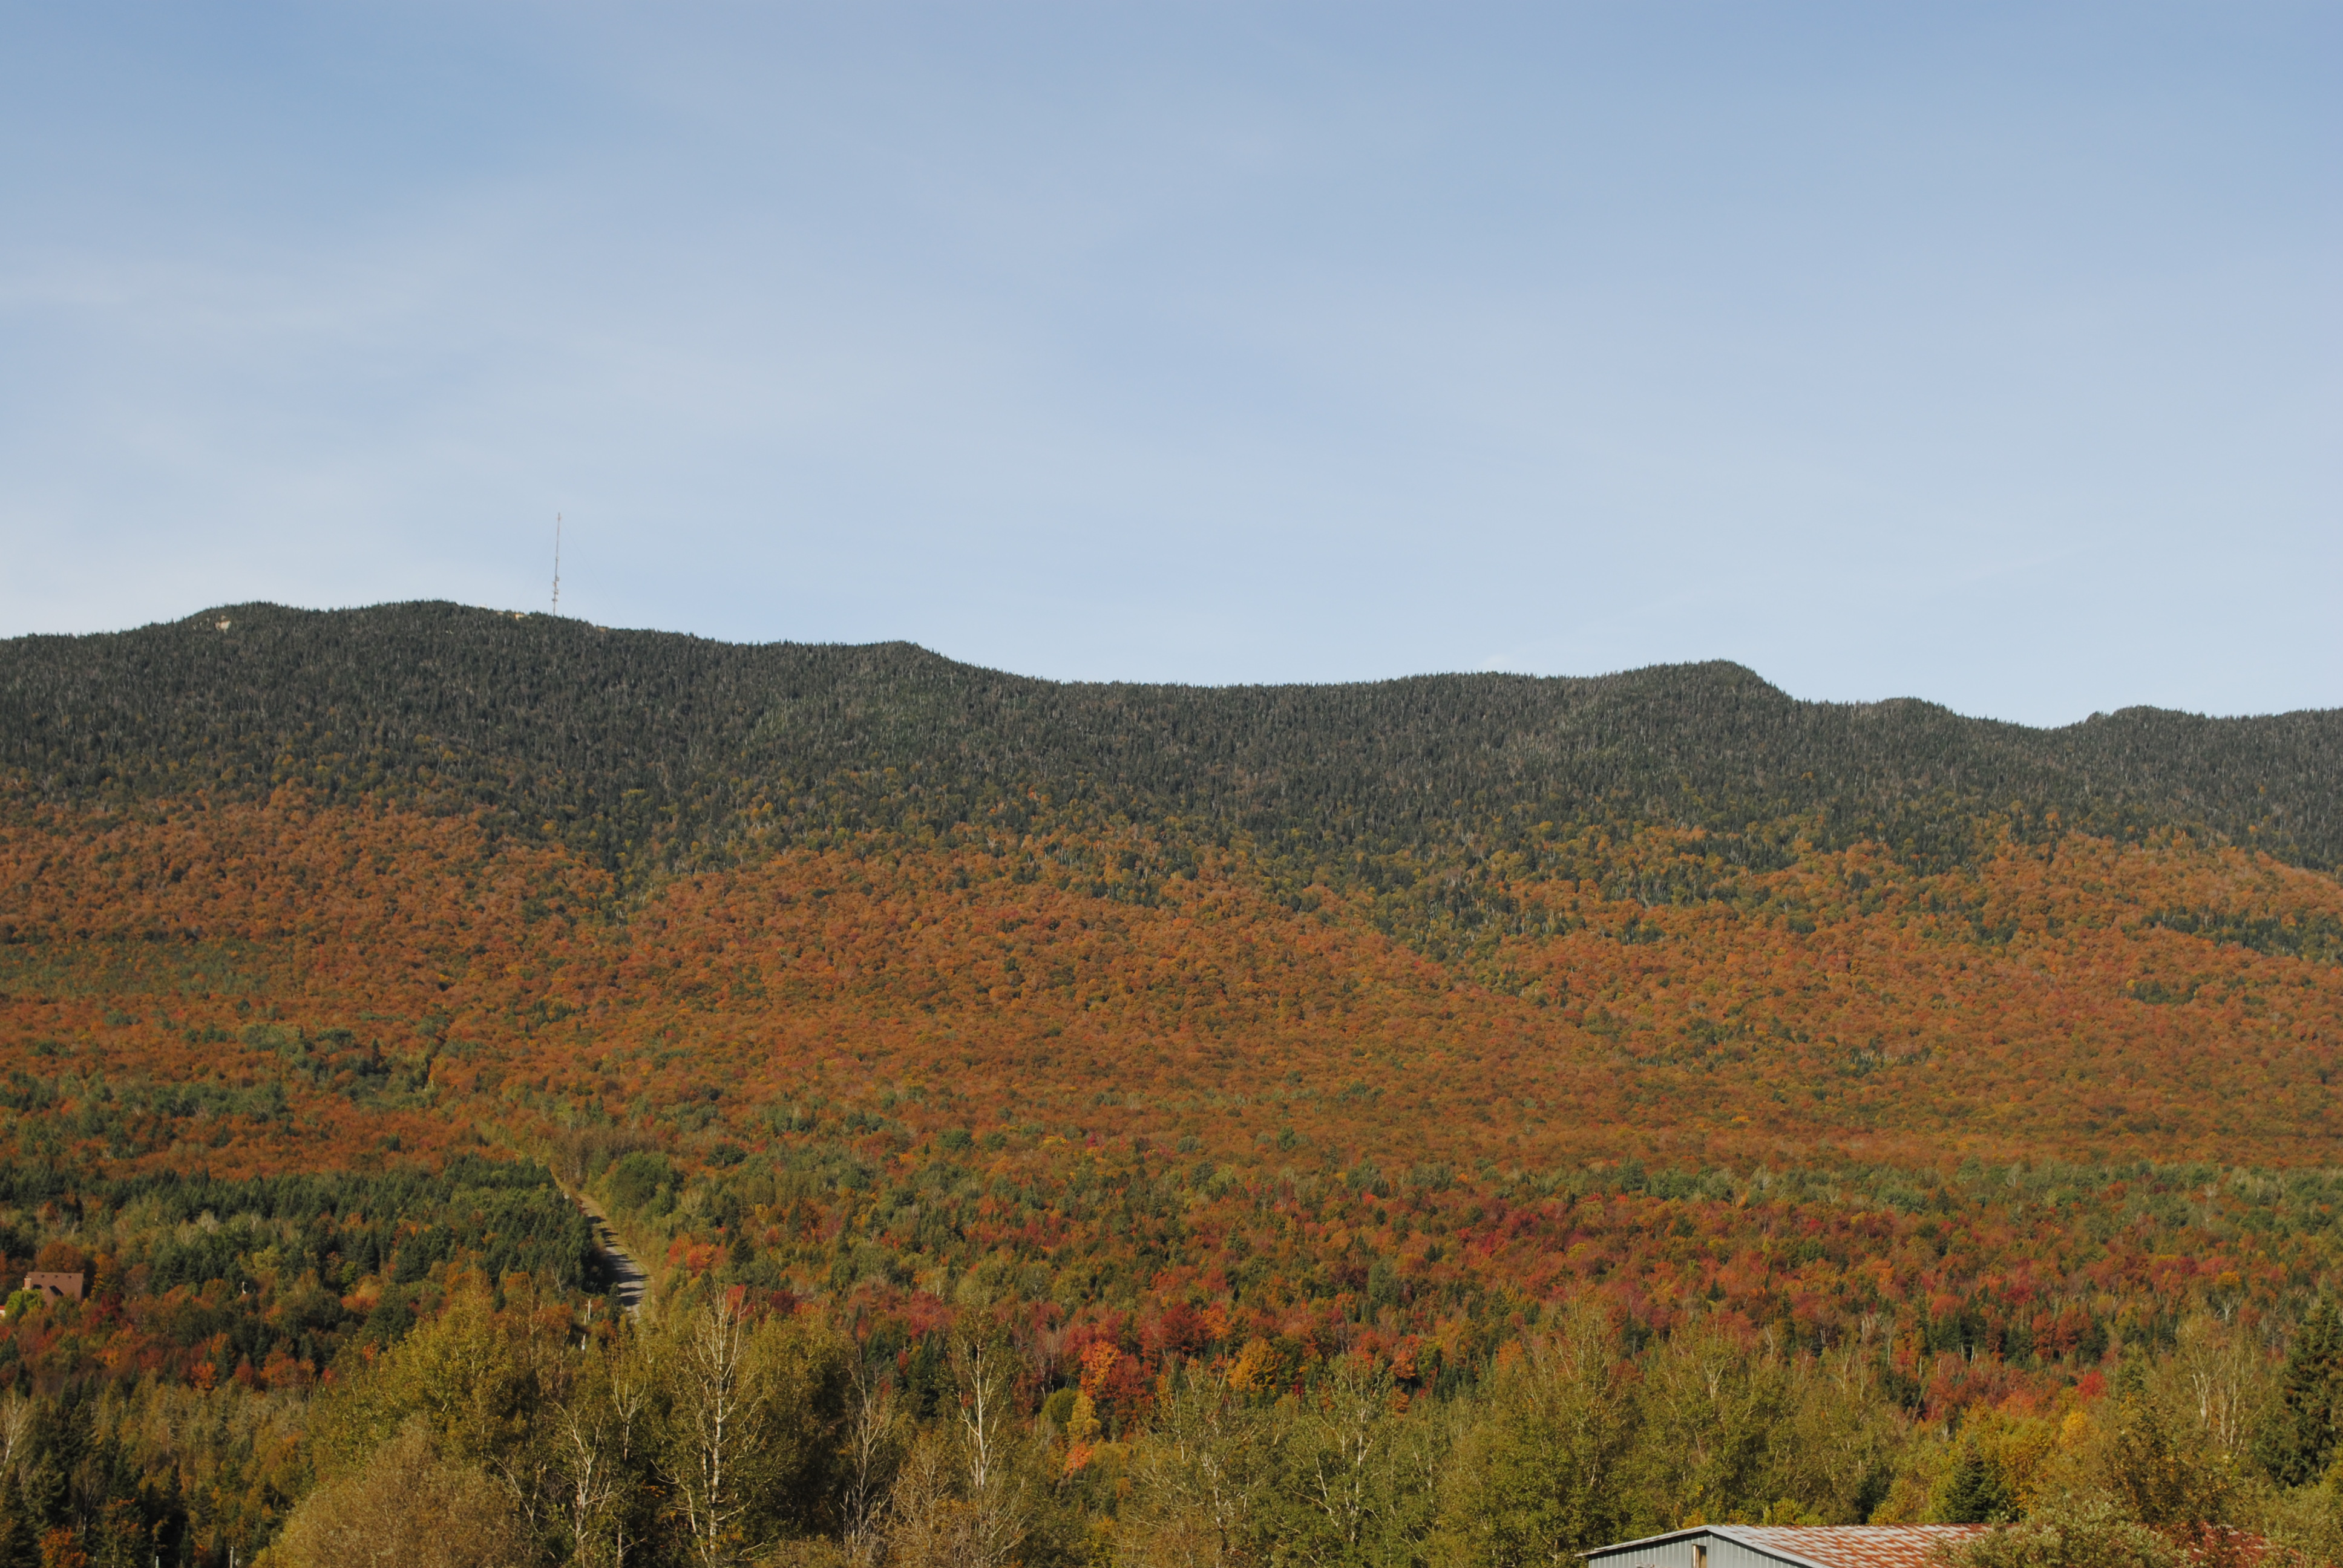
\includegraphics[height=0.65\textheight]{Figs/megantic}
    \end{center}

\end{frame}

%------------------------------

\begin{frame}{Islands}

    \begin{center}
        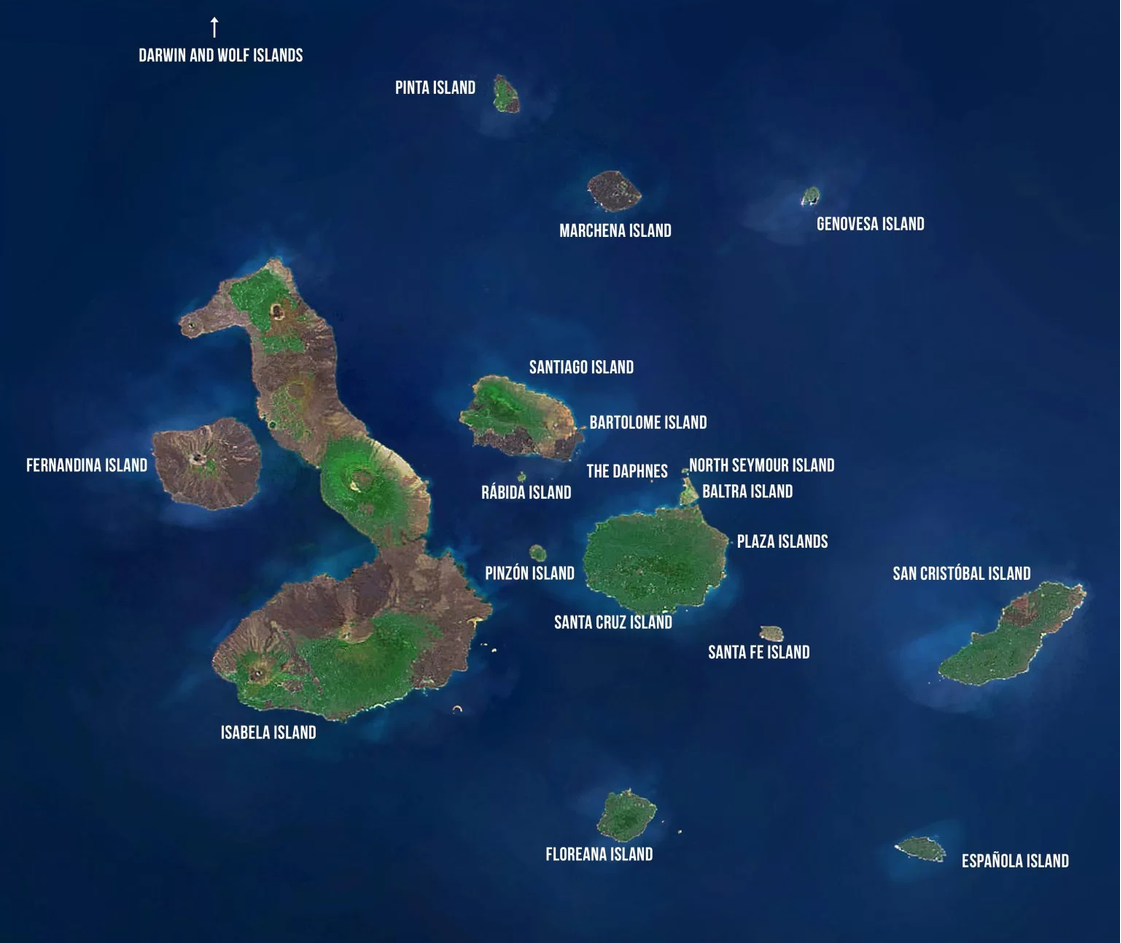
\includegraphics[height=0.7\textheight]{Figs/islands}
    \end{center}

\end{frame}

%------------------------------

\begin{frame}{Spatial structures}

    \begin{center}
        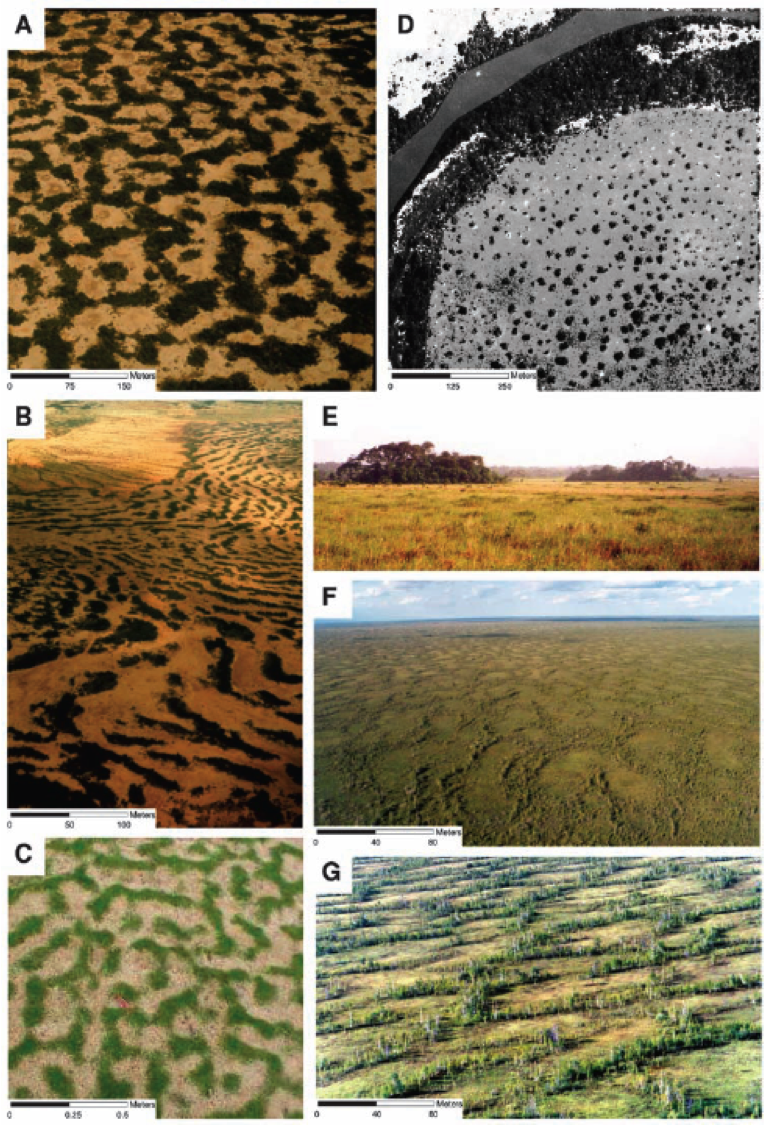
\includegraphics[height=0.8\textheight]{Figs/rietkerk2004}
    \end{center}

\end{frame}

%------------------------------

\begin{frame}{Coexistence}

    \begin{center}
        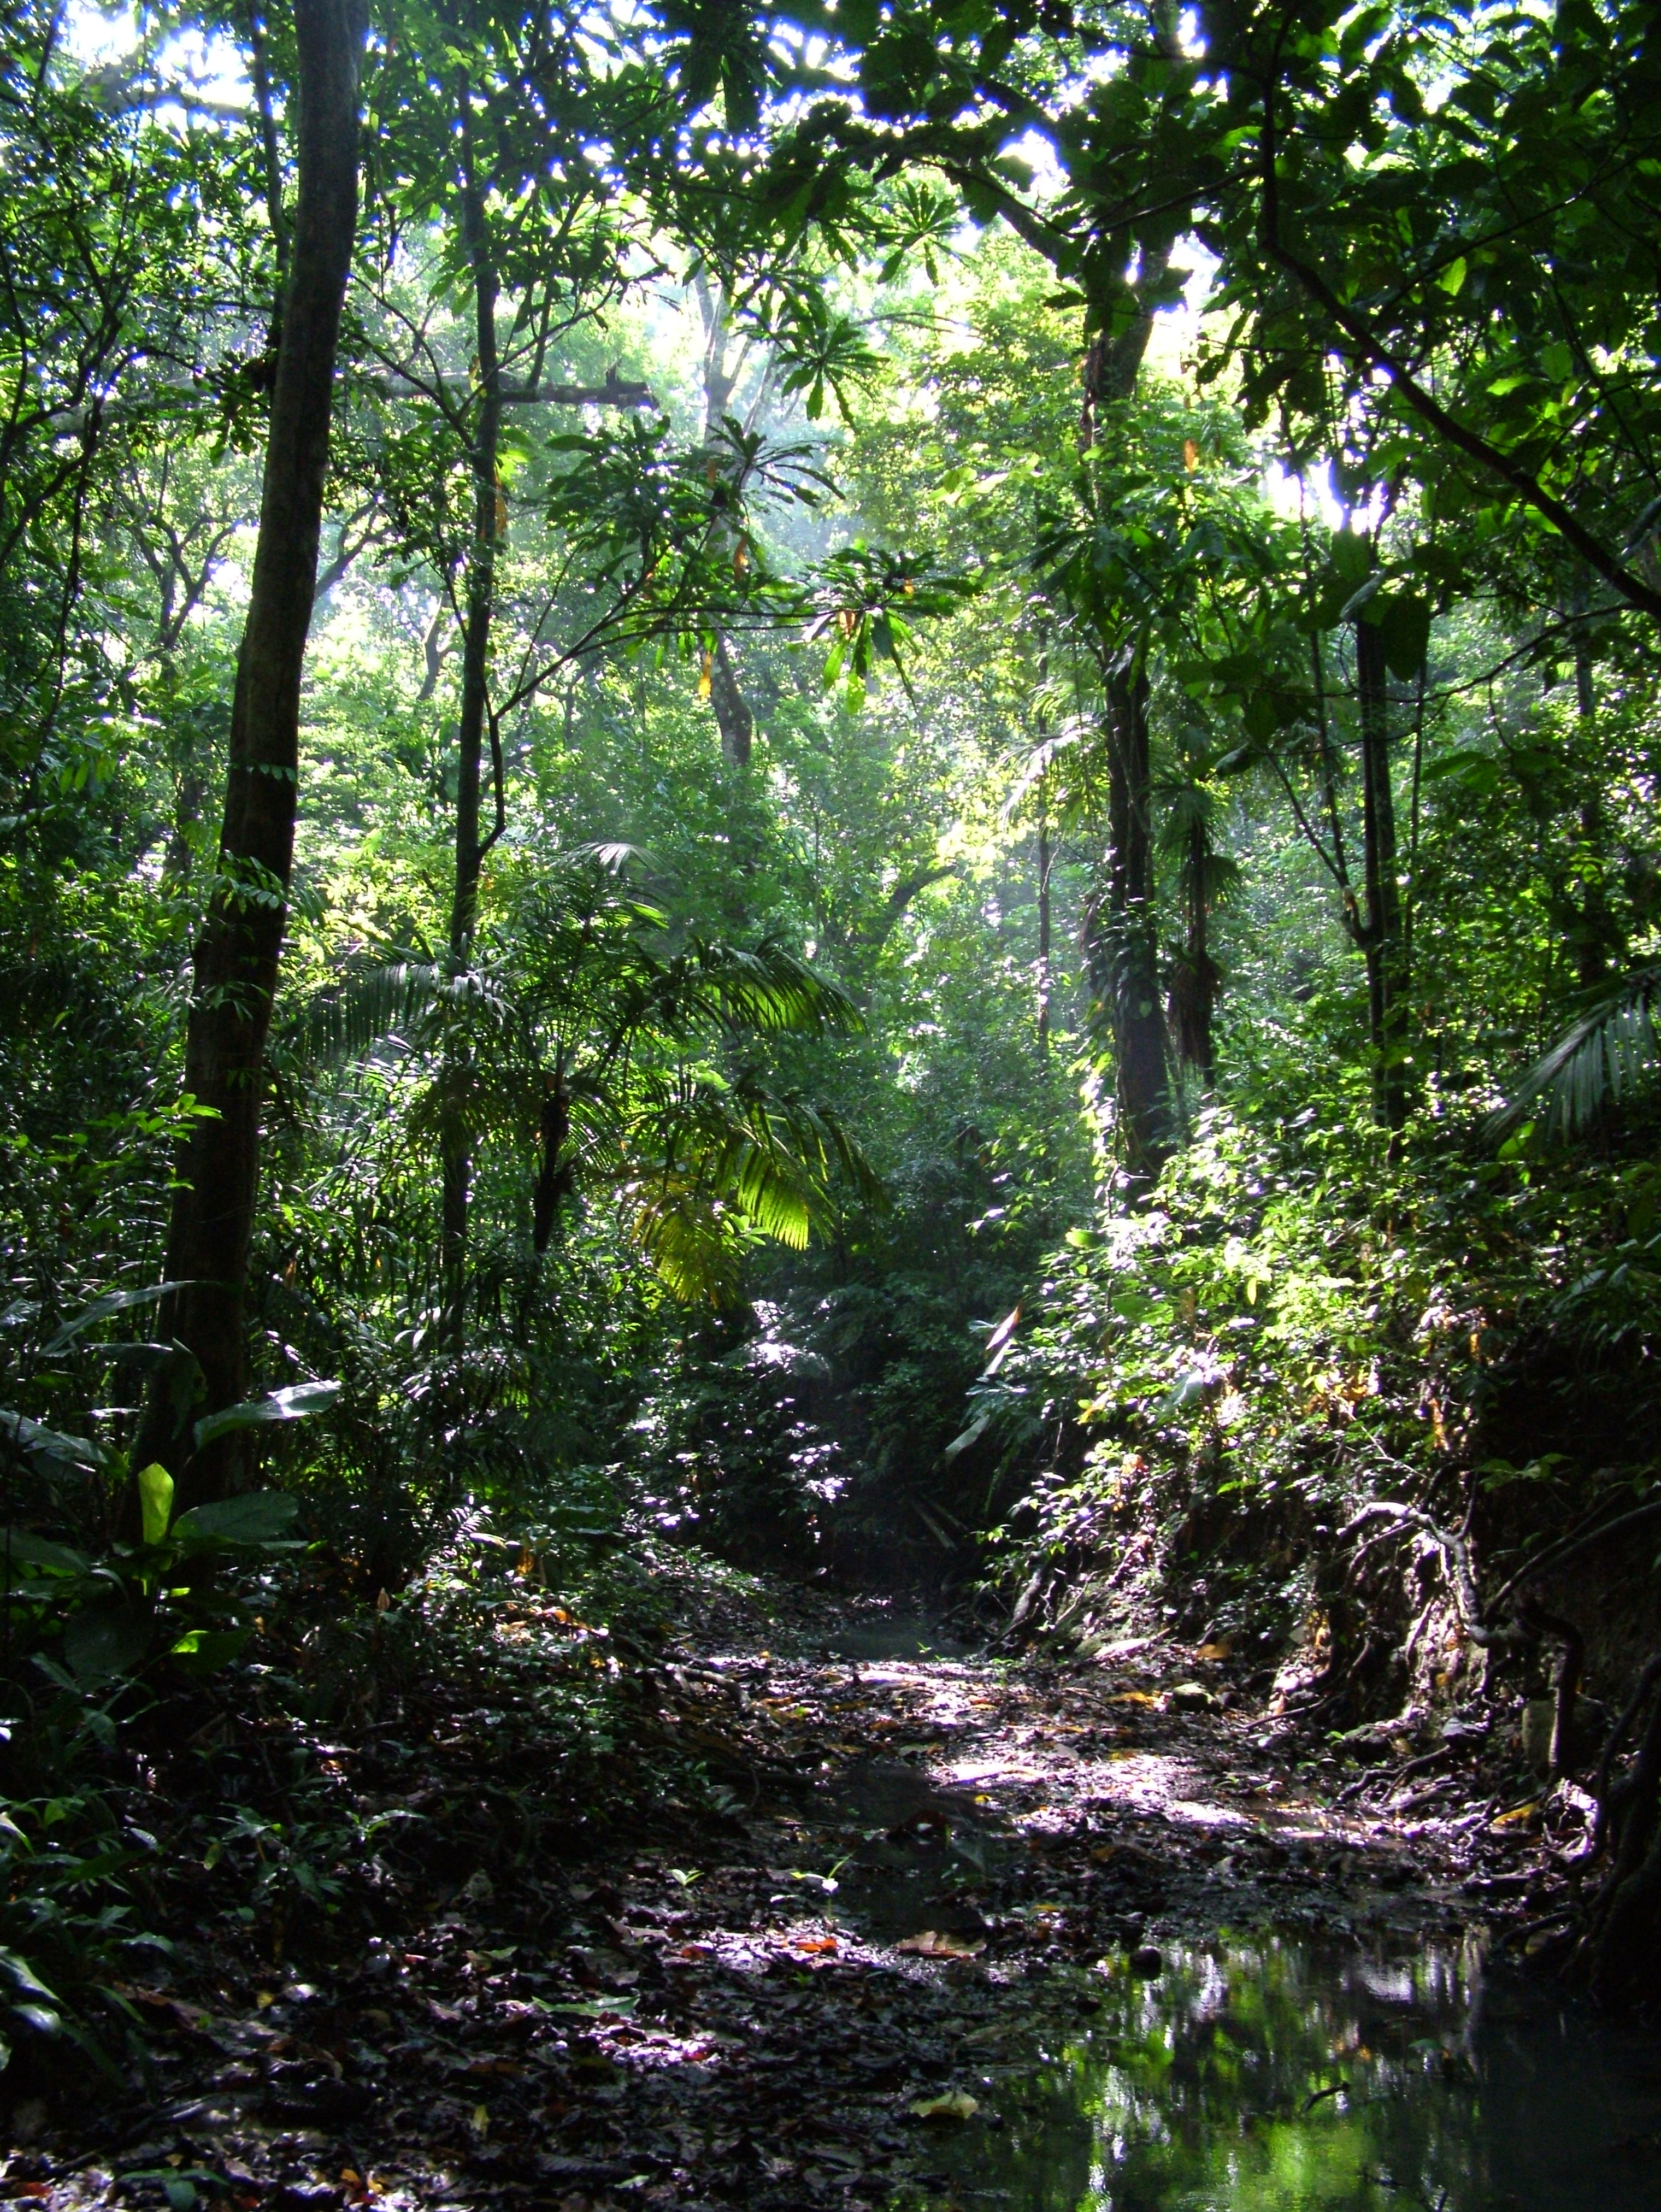
\includegraphics[height=0.8\textheight]{Figs/tropics}
    \end{center}

\end{frame}

%------------------------------

\begin{frame}{Spatial interactions}

    \begin{center}
        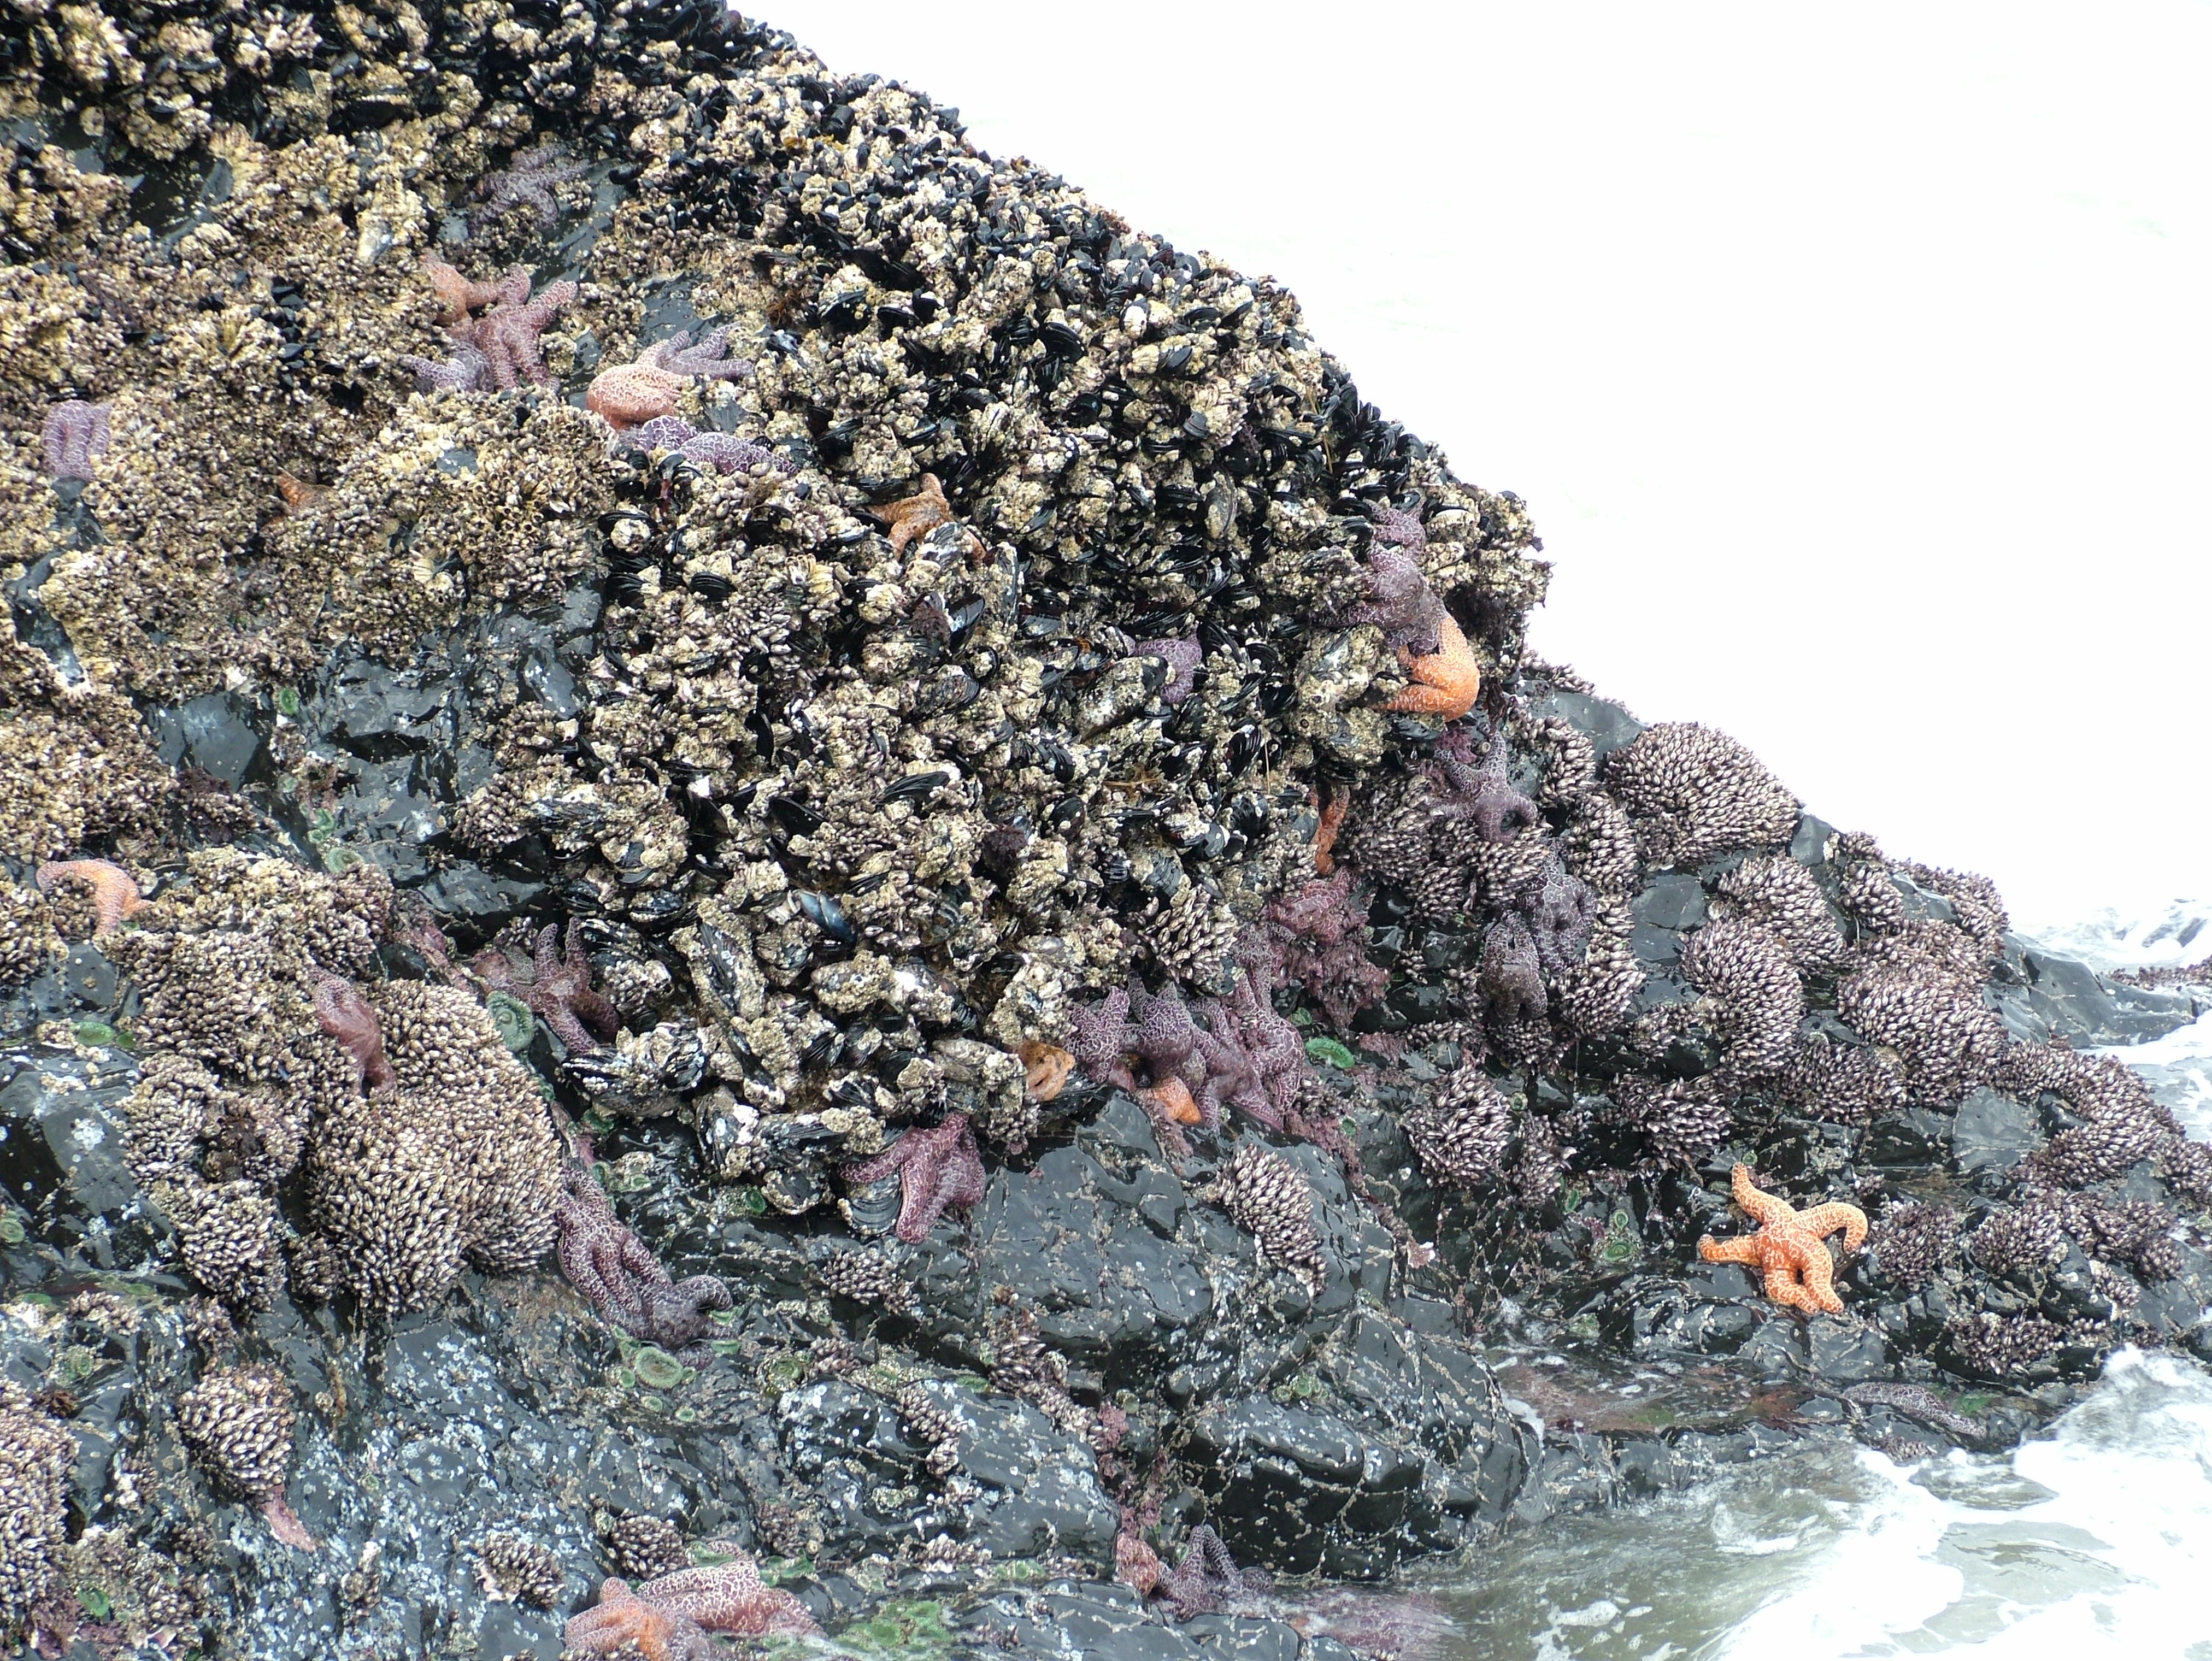
\includegraphics[height=0.7\textheight]{Figs/interactions}
    \end{center}

\end{frame}

%------------------------------

\begin{frame}{Fragmentation}

    \begin{center}
        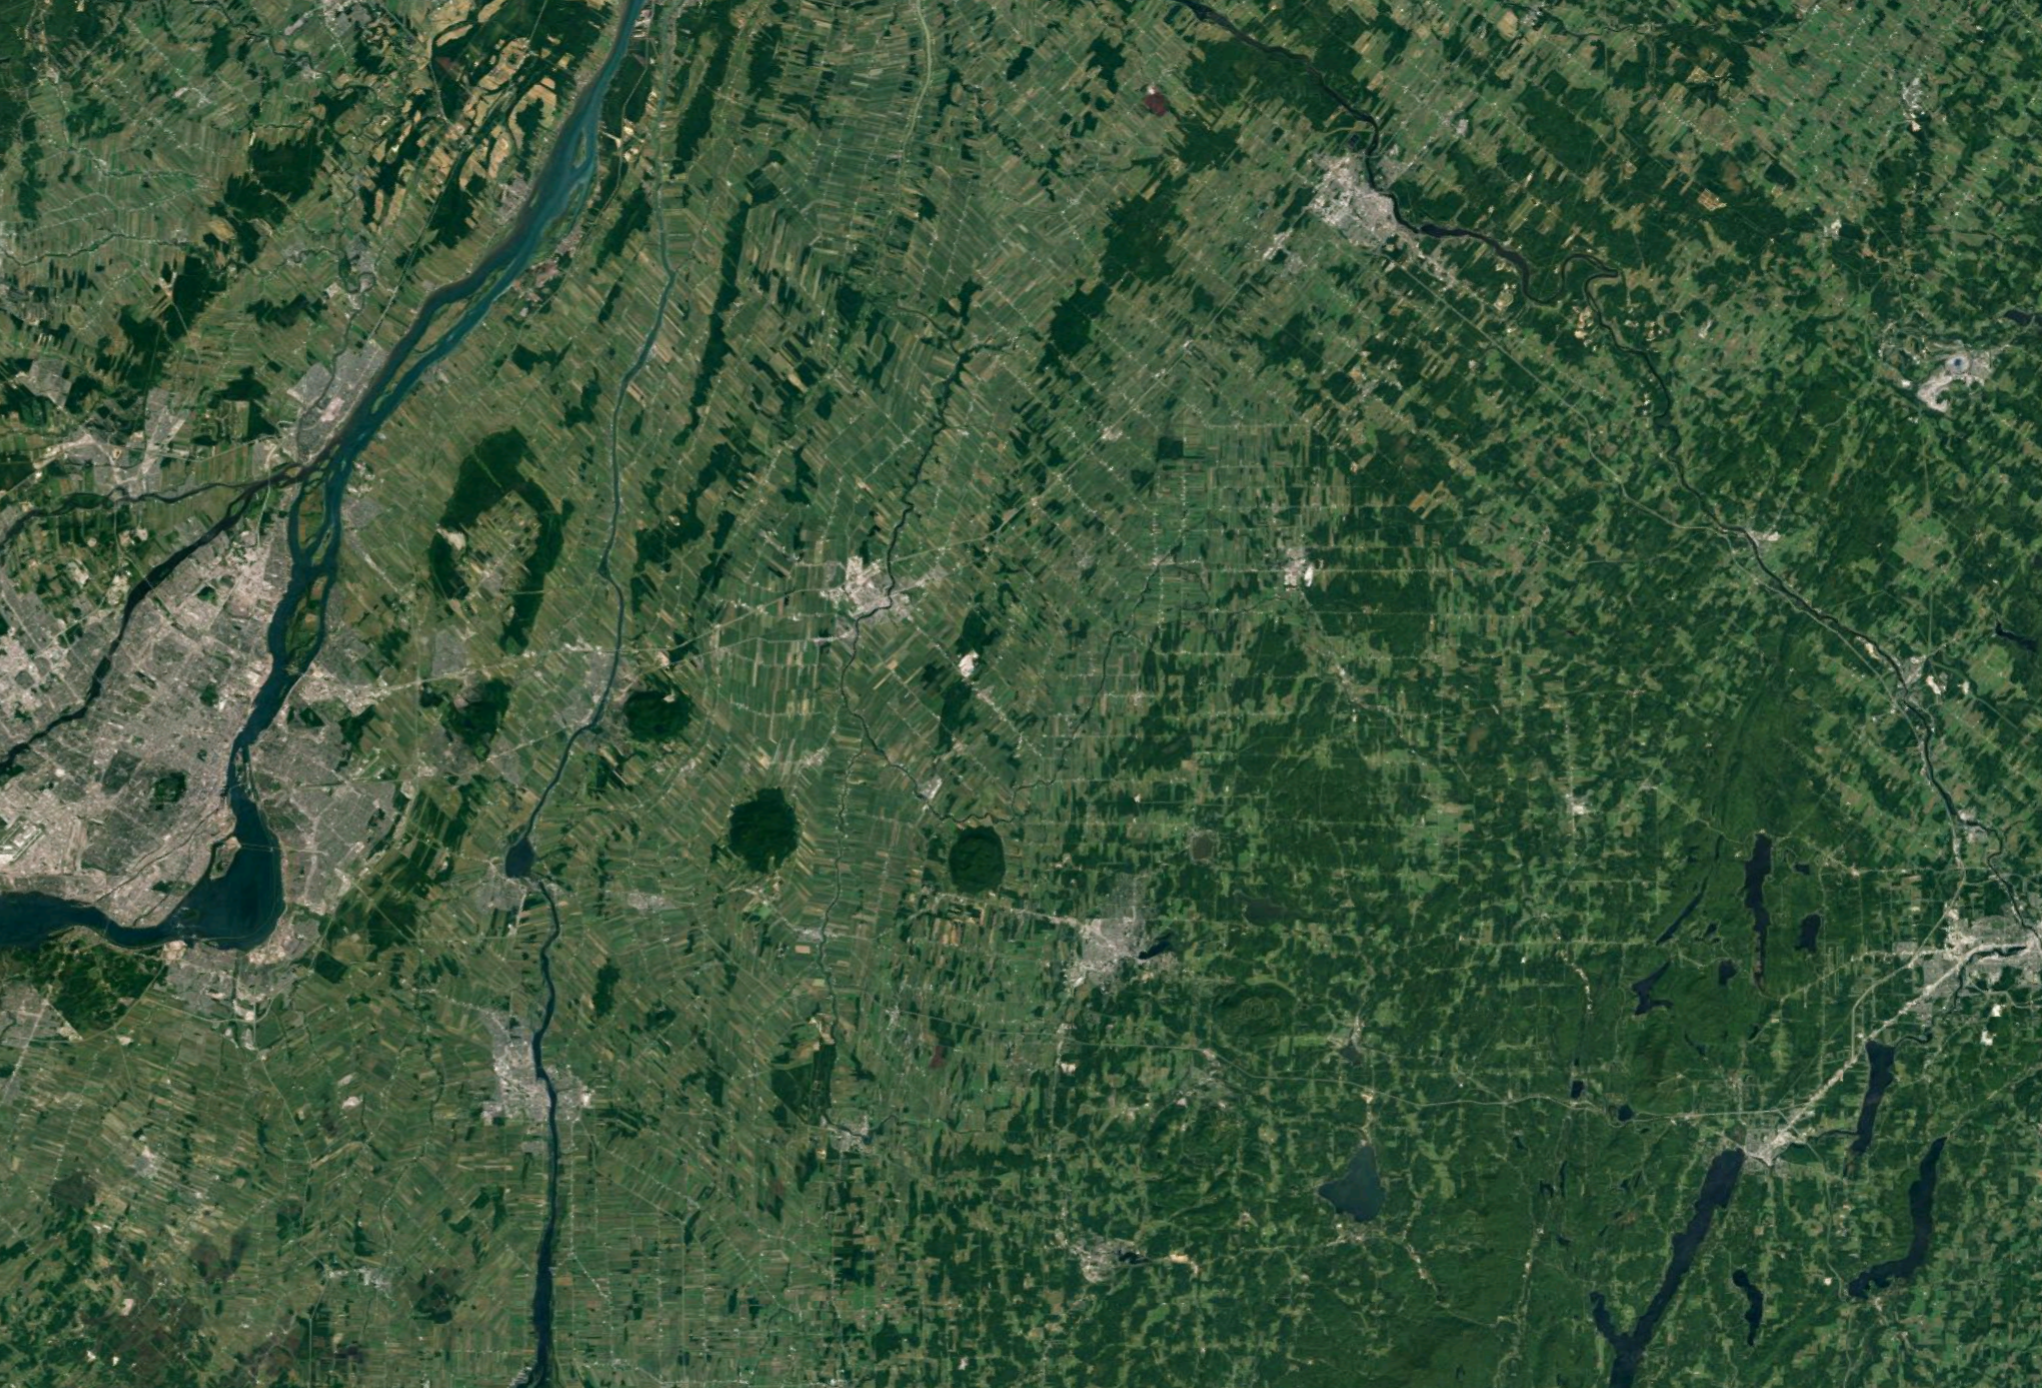
\includegraphics[height=0.7\textheight]{Figs/fragmentation}
    \end{center}

\end{frame}

%------------------------------

\begin{frame}{Corridors}

    \begin{center}
        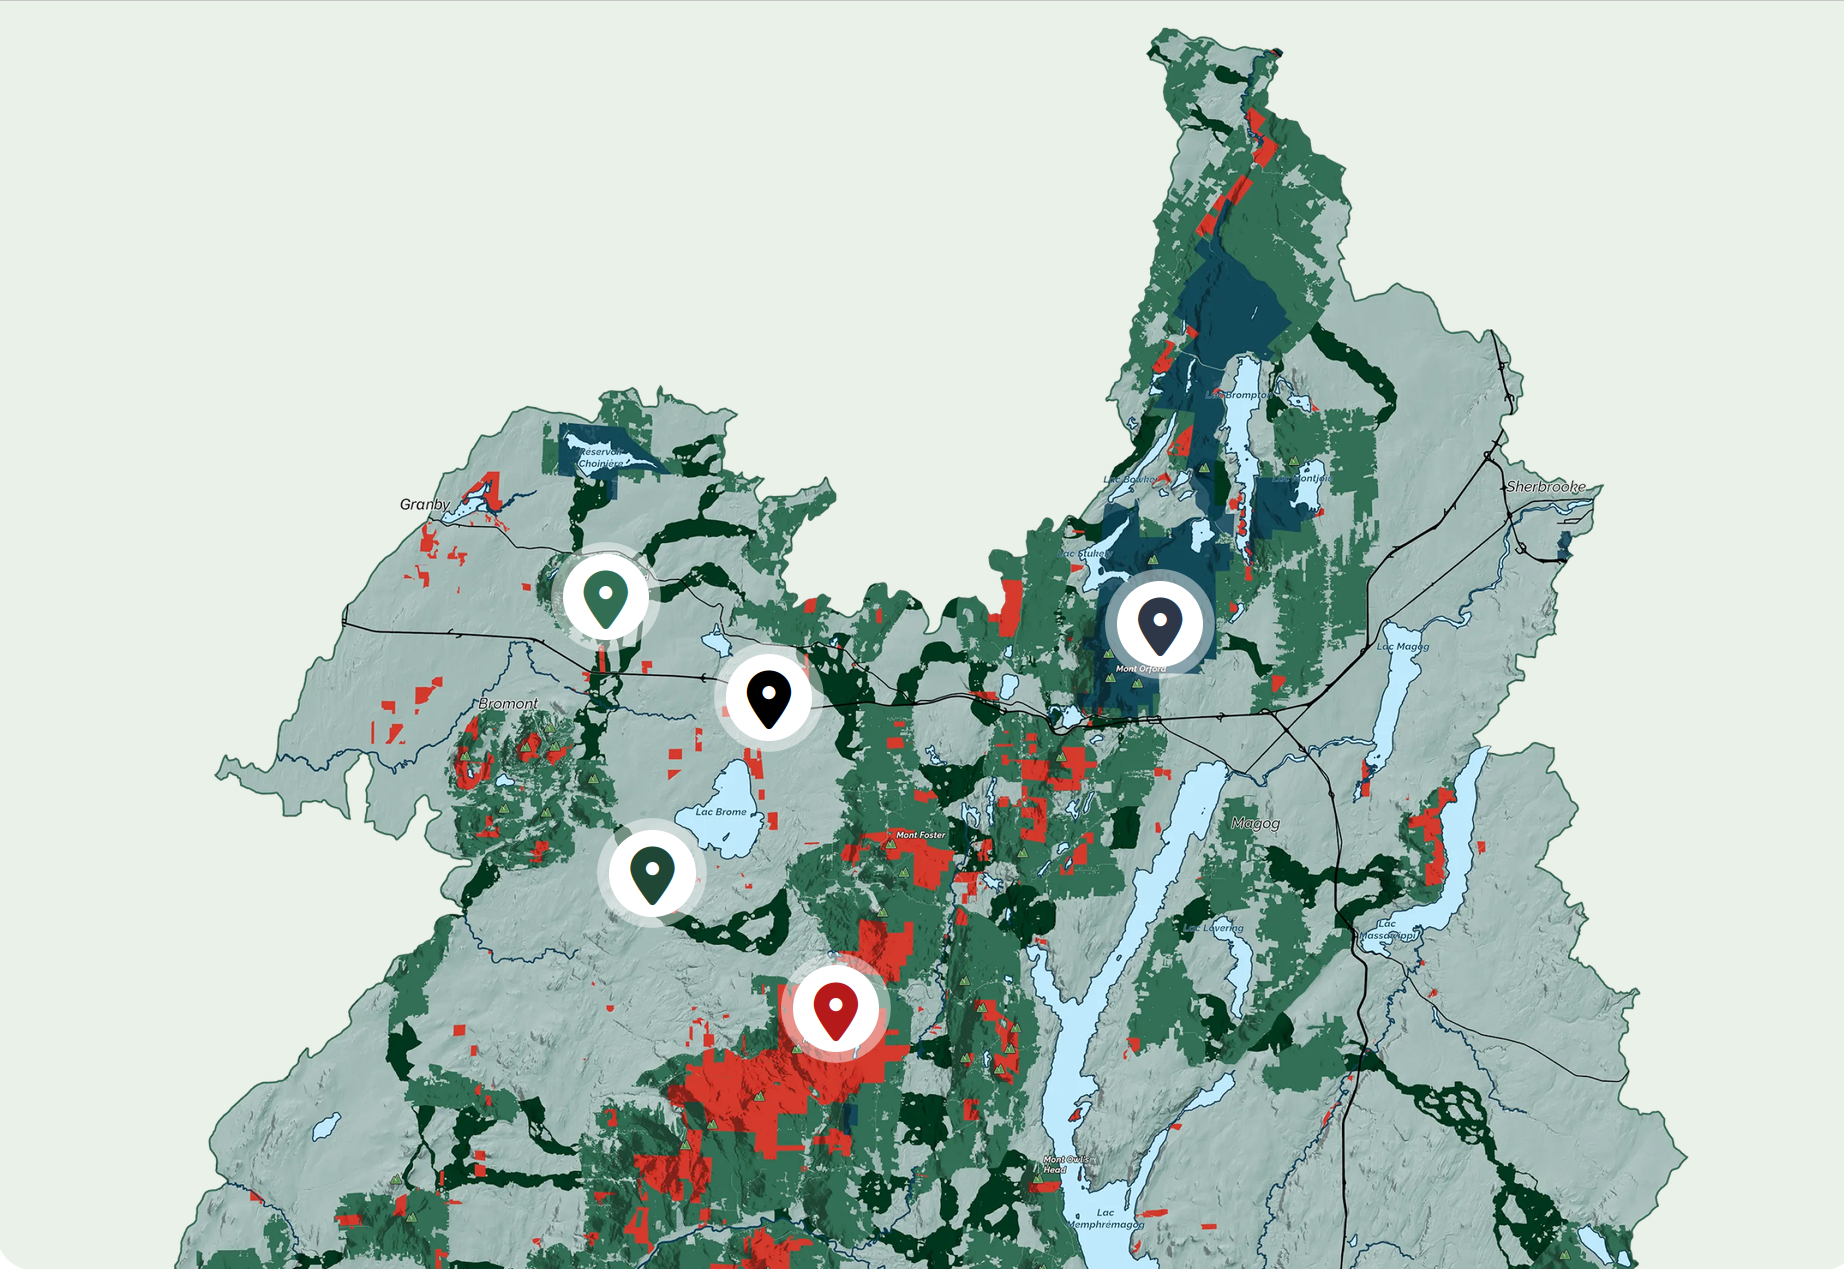
\includegraphics[height=0.7\textheight]{Figs/corridor}
    \end{center}

\end{frame}

%------------------------------

\begin{frame}{Migration}

    \begin{center}
        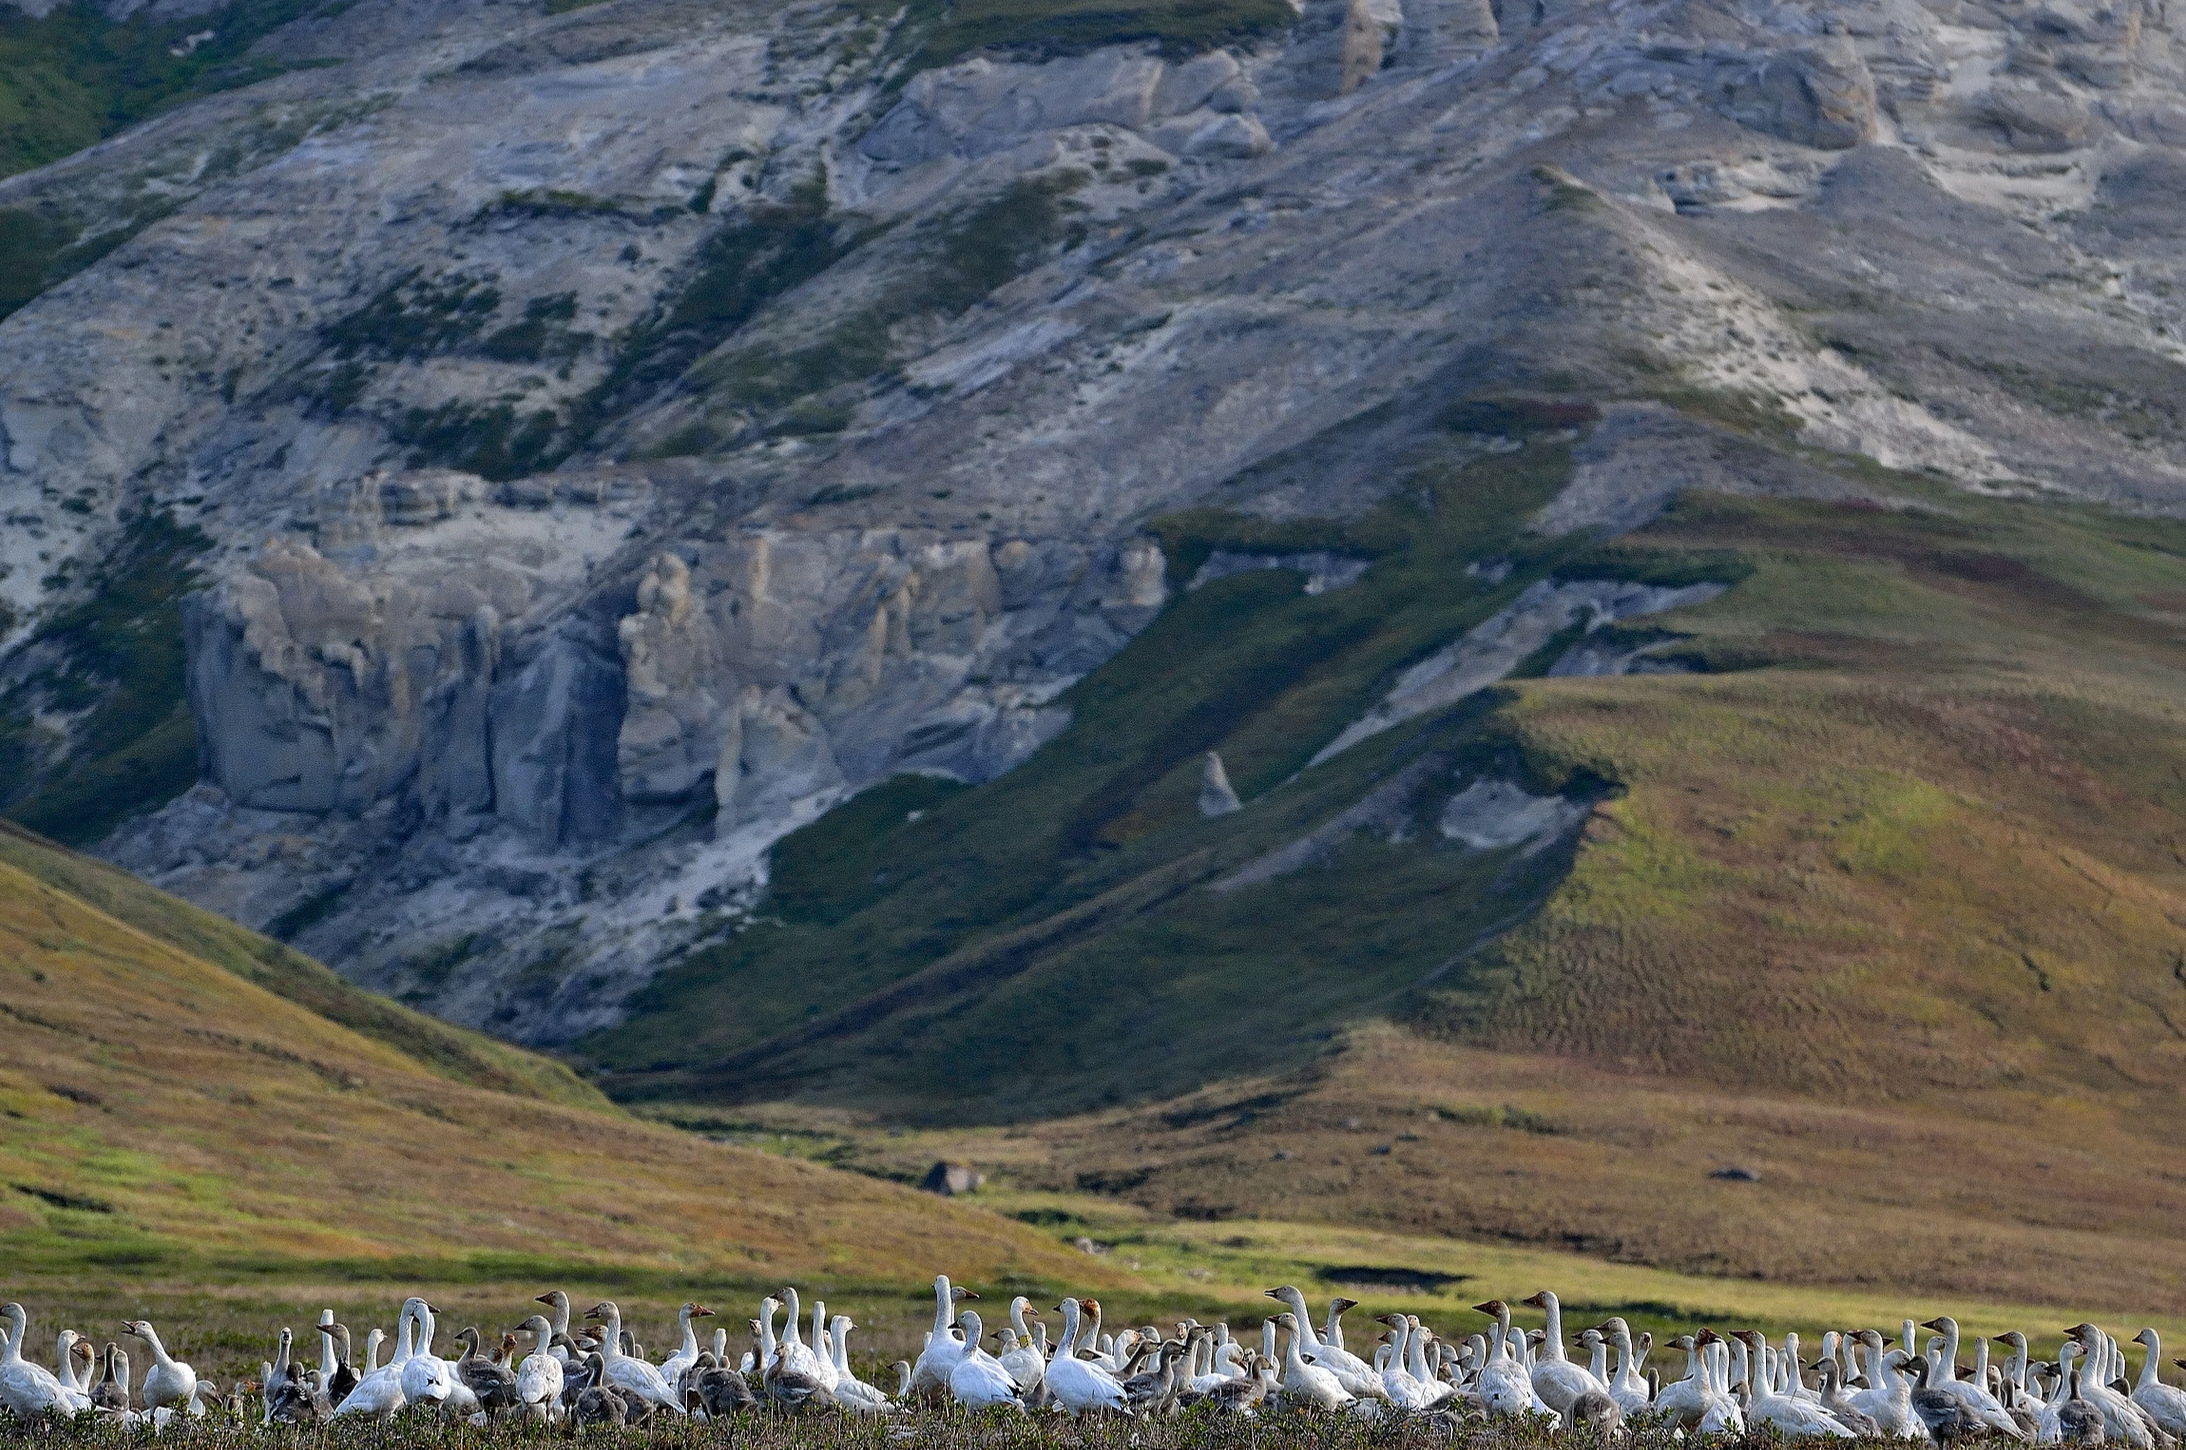
\includegraphics[height=0.7\textheight]{Figs/goose}
    \end{center}

\end{frame}

%------------------------------

\begin{frame}{Objectives}

    \begin{itemize}
        \item Overview of the main theoretical frameworks in spatial ecology 
        \item Explore modelling techniques for theoretical, simulation and statistical problems
        \item Build on this knowledge to explore novel questions in biodiversity science 
    \end{itemize}

\end{frame}

%------------------------------

\begin{frame}{Day 1}{Movement ecology}

    \begin{itemize}
        \item Course presentation
        \item Historical overview of spatial ecology
        \item From individuals to collective behaviour
        \item Minimal ingredients for emerging home ranges 
        \item Discussion on current topics in spatial ecology
    \end{itemize}

\end{frame}

%------------------------------

\begin{frame}{Day 2}{Metapopulation}

    \begin{itemize}
        \item Spatially implicit vs explicit metapopulations
        \item Pattern formation in dynamic metapopulations
        \item Realistic landscapes
        \item Persistence in spatial networks
        \item Promises and limits of Vibecoding spatial problems
        \item Model conception
    \end{itemize}

\end{frame}

%------------------------------

\begin{frame}{Day 3}{Metacommunity 1}

    \begin{itemize}
        \item The importance of dispersal for community structure
        \item Pedro Peres-Neto, Beta diversity in metacommunities 
        \item A neutral baseline for metacommunity dynamics
        \item Simulating neutral dynamics
        \item Breaking neutrality with lottery models
        \item Simulations
    \end{itemize}

\end{frame}

%------------------------------

\begin{frame}{Day 4}{Metacommunity 2}

    \begin{itemize}
        \item Fundamental spatial constraints on food webs
        \item Network-area relationship
        \item Dispersal stabilizes predator-prey interactions
        \item Reaction-diffusion in predator-prey models 
        \item Handling spatial objects in R 
        \item Figures \& analysis
    \end{itemize}

\end{frame}

%------------------------------

\begin{frame}{Day 5}{Metaecosystem}

    \begin{itemize}
        \item Spatial cascades in meta-ecosystems
        \item Indirect interactions
        \item Presentation of results        
    \end{itemize}

\end{frame}

%------------------------------

\begin{frame}{Evaluation}

    Evaluation (Pass or Fail) is based on participation to the different activites of the week. 

\end{frame}

%------------------------------
%------------------------------
\end{document}
